\subsection{SOAP/BPEL Web Service}

BPEL (the business process execution language) is an entirely Web Services based language that offers flexible coupling between several systems. Moreover,  Web Services are based on XML and they provide means of communication over a network in an open and flexible way. The objective all of these technologies is to automate process executions across system and the client. BPEL specification was written by Microsoft, IBM, and BEA and it consists of web services definition language (WSDL) files defining the underlying Web Services and BPEL files defining the entire business process. All BPEL processes have only one variable variable (which, in our case, would be the \textit{itinerary}). 

BPEL process indicates the order in which Web services should be invoked. There was used <receive> and <reply> blocks in order to interact with the client and initiate the logic for the operations he performed. There was also used <assign> blocks to convert one complex types to another in order to <invoke> simple web services, that have been used in intermediate steps. There was also used <flow> mechanism to run in parallel during booking and cancelling itinerary to speed up the process (instead of sequential operations). For exception handling and tractionality for core operations, there were used <scope> and <compensationhandler> as well as <faulthandler> in each scope. Details of the BPEL process are being discussed below in further sections.
The BPEL process starts when a client requests to create an itinerary using \textit{createItineraryOperation} which expects a user id as input and returns itinerary id as output. The uniqueness of an itinerary was enforced by the BPEL process itself using correlation sets. Whenever a user requests to create an itinerary, we create a GUID as itinerary id and correlate the whole business process using that id meaning that each subsequent operation calls will contain the itinerary id in their input in order to figure out which BPEL process they are on. 

After itinerary is created, we step into \textit{planning phase} which contains two different scopes namely \textit{booking scope} and \textit{waiting scope}. In the booking scope, client can get possible flights/hotels according to his/her needs and adds them into his/her itinerary. The scope terminates when the user calls \textit{bookItineraryOperation} with a credit card info. 
After the itinerary is booked, we enter into waiting scope where the process waits until the first date of the booked flight/hotel in the itinerary and terminates the whole process when the time exceeds.

In the whole planning phase, the client can call \textit{getItineraryOperation} in order to see the current status of the itinerary or the client can call \textit{cancelItineraryOperation} that will terminate the whole process if the itinerary is not booked, or it will wait until the first date of the flight/hotel in the itinerary before it terminates the whole process. The overall abstract representation of TravelGood BPEL implementation is shown in figure~\ref{fig:abstract-representation}.

\begin{figure}[H]
\centering
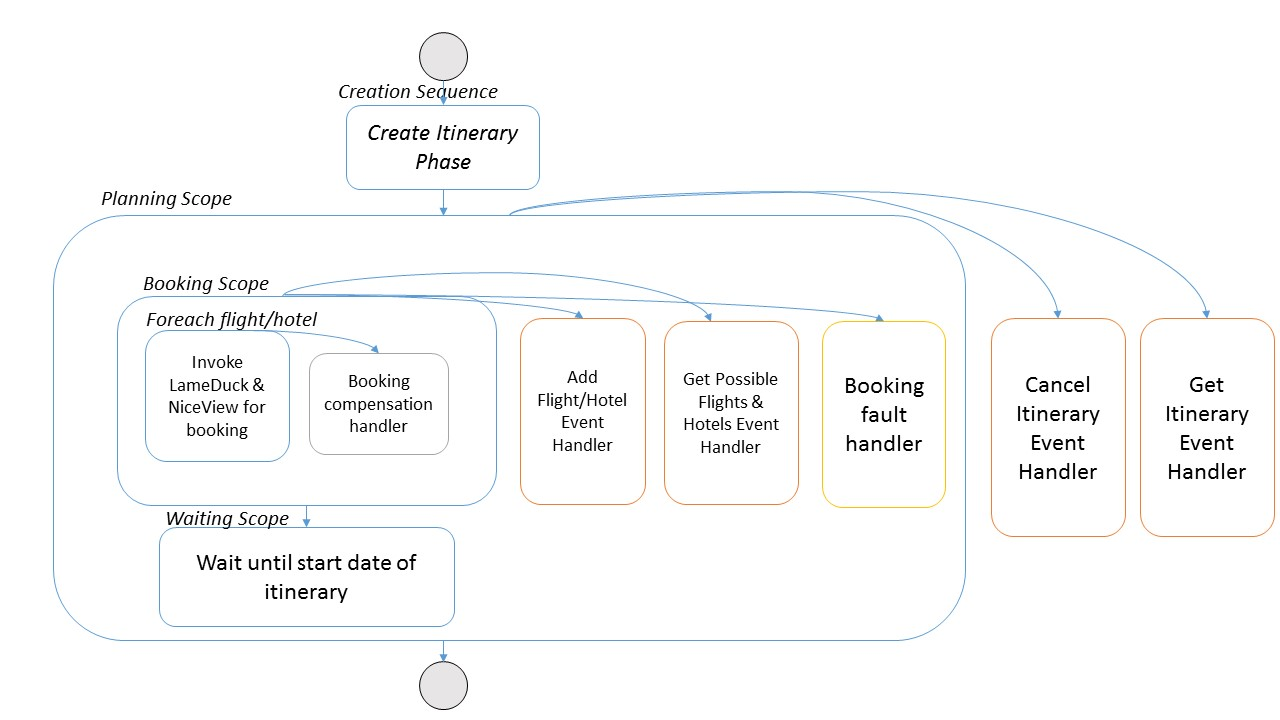
\includegraphics[width=0.9\textwidth]{images/bpel_abstract_impl.jpg}
\caption{Abstract representation of TravelGood BPEL implementation.} \label{fig:abstract-representation}
\label{statediagram}
\end{figure}

\subsubsection*{Create Sequence}
BPEL uses a sequence approach to web services with a visual interface to go along with it. To start our BPEL process, the client sends a request to the \textit{createItineraryOperation}() taking a string representing the ID of the client as input and returning another string representing the ID of the created itinerary as a result. Using this ID, the correlation set of the BPEL process is initiated and all the subsequent operation calls will contain the itinerary ID as an input. In this way the BPEL engine is able to understand the current execution order of the process and can easily distinguish between different processes. Before returning the ID of the created itinerary, empty lists are assigned  to \textit{flightInfoArray} and \textit{hotelInfoArray} variables, part of the itineraryInfo variable in the create sequence and the value of the current booked variable is set to false. After the unique identifier is returned to the client, the creation sequence is finished and the process enters the planning scope.

\subsubsection*{Planning Scope}

At any time in the planning scope the customer can cancel the itinerary and get the current state of itinerary.

\textbf{\textit{Cancel Itinerary Event Handler}}

According to the requirements, clients have the possibility to cancel planning phase as well as booking. A \textit{cancelItineraryOperation} expects the itinerary ID and a credit card information as an input and returns true or false, depending on if the cancellation is successful or not. At the beginning  of a scope associated with \textit{CancelItinerary} event, a variable called \textit{cancelItineraryOutput} is defined with a boolean true value assigned to it. This variable is used to determine if the cancellation was successful or not at the end of the scope.

There are two possible actions - client cancels either during planning or booking - so there are two If activities \textit{IfBooked} and \textit{IfNotBooked}. To determine which activity should be used, the process checks value of the variable \textit{booked} (true or false). Variable \textit{booked} is set to false when the process starts and is set to true after booking phase finished successfully. The abstract representation of TravelGood cancel itinerary event handler is shown in figure~\ref{fig:abstract-cancel}.

\underline{\textit{IfBooked activity}}

The implementation of this activity is based on two parallel flows, one for cancelling flights and the second one for cancelling hotels. Both tasks are independent since they use two different external web services. By using two separate ForEach activities, the process goes through all of the items in \textit{flightInfoArray} and \textit{hotelsInfoArray} respectively, it is through all of the items in the itinerary.

The flow in each of \textit{ForEach} activity is as follows:
take current element from an array and assign it to the \textit{currentFlightInfo/ currentHotelInfo} variable,
assign necessary values to the input variable for the external web service (booking number and credit card information),
invoke\textit{ LameDuck/NiceView} web service which are added as PartnerLinks,
make a logical AND operation of variables \textit{cancelItineraryOutput} and value returned from the web service and assign the result back to \textit{cancelItineraryOutput},
if the cancellation was successful then change the status of the current flight/hotel in an itinerary to CANCELLED.

Since cancelling may fail, there is a FaultHandler associated with a \textit{CancelFlightScope/ CancelHotelScope}. It is a \textit{catchAll} element which means than it catches all faults which occur in this scope. It handles exception which may be returned by the invoke activity and it assigns a logical false to \textit{cancelItineraryOutput} variable. It ensures that a logical false is returned whenever an invocation of cancel operation fails. 

After \textit{IfBooked} activity is finished, it replies with the value in \textit{cancelItineraryOutput} which is either true or false. True means that all of the booked items has been cancelled and false means that at least one of the booking has not been cancelled.

\underline{\textit{IfNotBooked activity}}

In case a client cancels a planning phase, a BPEL process replies with boolean true immediately. After that the BPEL process ends.

\begin{figure}[H]
\centering
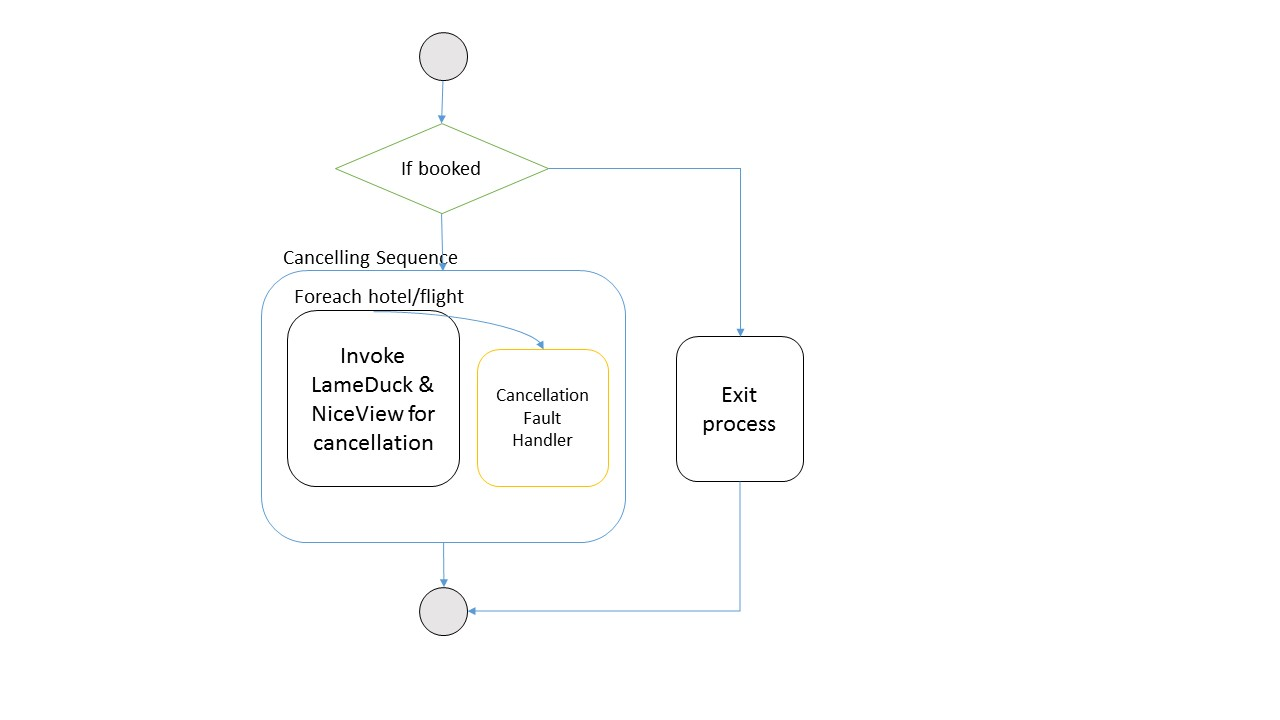
\includegraphics[width=0.8\textwidth]{images/bpel_cancel_abstract_impl.jpg}
\caption{Abstract representation of TravelGood cancel itinerary event handler.} \label{fig:abstract-cancel}
\label{statediagram}
\end{figure}

\textbf{\textit{Get Itinerary Event Handler}}

In the planning scope, the client is able to get the status of the itinerary anytime he wants. The event \textit{getItinerary} has an underlying scope in the event handler, named \textit{GetItineraryEventScope}, which assigns the itinerary info that we keep in the BPEL process to the \textit{getItineraryOutput} which contains \textit{flightInfoArray} and \textit{hotelInfoArray}.

\subsubsection*{Booking Scope}

At any time in the booking scope, the customer can get a list of possible flights and hotels for a destination and time as well as add flights and hotels to an itinerary. Hence, the events handled in this phase are:
\begin{itemize}
\item getting list of possible flights and hotels (\textit{getPossibleFlights/getPossibleHotels})
\item adding specific flight or hotel to itinerary (\textit{addFlight/addHotel})
\end{itemize}

\textbf{\textit{Get Possible Flights \& Hotels Event Handler}}

To get a list of possible flights one has to call the \textit{getFlight} operation from \textit{LameDuck} service. The \textit{getFlight} operation expects itinerary ID, departure airport, destination airport and departure date as input and returns an array (\textit{flightInfoArray}) with possible flights as output. The event \textit{getPossibleFlights} has an underlying scope in the event handler named \textit{GetFlightsEventScope}. The scope performs the following actions to return a list of possible flights to the client:
 
First it assigns the input for the \textit{getPossibleFlights} to the input for the \textit{getFlightsOperation} from the external service \textit{LameDuck}. \textit{LameDuck} is added as PartnerLink in BPEL.
Secondly the \textit{getFlights} operation from the \textit{LameDuck} service is invoked.
The list of flights from the \textit{LameDuck} service is then assigned to the \textit{getPossibleFlights} output in the \textit{TravelGood} web service. Hence, the output is a list of flights that satisfies the requirements specified by the client.
 
To get a list of possible hotels one has to call the gethotel operation from \textit{NiceView} service. The \textit{getHotel} operation expects itinerary ID, arrival date, departure date and city as input and returns an array (hotelInfoArray) as output. The event \textit{getPossibleHotels} has an underlying scope in the event handler named \textit{GetHotelsEventScope}. The scope performs the same actions as the scope for \textit{GetPossibleFlights}, but in this case it assigns to the input for the getHotel operation from the external service \textit{NiceView} and it assigns the response to the \textit{getPossibleHotels}. As LameDuck, \textit{NiceView} is added as a \textit{PartnerLink} in BPEL.


\textbf{\textit{Add Flight/Hotel Event Handler}}

The addFlight event expects the id of the itinerary and a flight info that is going to be added to itinerary and it returns \textit{FlightInfoArray} and \textit{HotelInfoArray} as output that shows the current itinerary. The scope for the event \textit{addFlight} is named \textit{AddFlightEventScope}. The scope performs the following actions:
 
It finds the number of flights already added to the itinerary and assigns the value to the \textit{numberOfFlights} variable.
The flight that should be added to the itinerary is then appended to the end of the list of flights in the itinerary (flightInfoArray), by using the \textit{numberOfFlights} variable.
The scope then returns the updates \textit{flightInfoArray} as well as \textit{hotelInfoArray}.

The \textit{addHotel} event expects itinerary ID and a \textit{hotelInfoType} as input and it returns \textit{FlightInfoArray} and \textit{HotelInfoArray} as output. The scope for the event \textit{addHotel} is named \textit{AddHotelEventScope}. The scope performs the same actions as the scope for \textit{addFlight}, but instead it finds the number of hotels already added to the itinerary and assigns the value to the \textit{numberOfHotels} variable. The hotel that should be added to the itinerary is then appended to the end of the list of hotels in the itinerary (hotelInfoArray).   


\textbf{\textit{Booking operation}}

The BPEL process enters the booking phase when the \textit{bookItinerary()} operation is called by the client. The sequence starts by retrieving the information received from the client and required for the booking operation: an \textit{itinerary} and \textit{credit card information}.  After this, the following flow of activities in \textit{BookingFlow} is triggered:
\begin{itemize}
\item the process iterates through both the flights and the hotels arrays and enters a new scope for every iteration (\textit{BookFlightScope / BookHotelScope}),
\item in each of these inner scopes the following sequence of activities is executed:

\begin{itemize}
\item assign the values of the flight/hotel object from the received itinerary to the \textit{currentFlight/curentHotel} variable,
\item assign the values of the {currentFlight/curentHotel} variable to an input variable that will be used to invoke the \textit{bookFlight()/bookHotel()} operations from \textit{LameDuck/NiceView} external services (these are added as PartnerLinks in BPEL and can be called at any time throughout the process),
\item invoke the booking operation from the external web services,
\item assign the result of the invoke activity to the result of the \textit{bookItinerary()} operation,
\item change the status of the flight/hotel object in the current iteration to ''CONFIRMED''.
\end{itemize}

\end{itemize}

Both inner scopes discussed above can terminate with a fault since both \textit{bookFlight()} and \textit{bookHotel()} operations of \textit{LameDuck} and NiceView services return a fault if errors occurred during booking; in BPEL, these faults are handled using FaultHandlers. We set the fault handler in the booking scope so that whenever a fault is thrown in a booking invocation, we will catch it in the scope and by using Compensate activity, we start to compensate all the successfully finished subscopes.

In addition, whenever a fault occurs, the booking operation needs to compensate for the flights/hotels that have already been booked and revert everything (refund, if necessary). In BPEL, compensation is achieved using CompensationHandlers, therefore, each of the inner scopes have their own compensation handler executing the following sequence of activities:

\begin{itemize}
\item assign the values of the \textit{currentFlight/currentHotel} variable to an input variable that will be used to invoke the \textit{cancelFlight()/cancelHotel()} operations from \textit{LameDuck/NiceView} extrenal services,
\item invoke the cancelling operation from the external web services. Since cancellation logic for flights includes only refunding half of the price that is paid by booking, when we are invoking cancelling operation in compensation handler, we call with the double amount of the booking price to ensure that it is refunded the whole amount,
\item change the status of the flight/hotel object in the current iteration to ''CANCELLED''.
\end{itemize}

After the sequences of activities from the inner scopes have finished successfully, the value true will be assigned to the global variable \textit{booked} (variable created when the process starts) and a reply is sent back to the client. 

The process is however not terminated yet, it enters a waiting state according to the logic described in the \textbf{Waiting Scope} section.

\subsubsection*{Waiting Scope}

The wait logic is used after the an itinerary has been booked, to keep the instance alive until the earliest itinerary item has passed. To do this we first loop through the \textit{flightInfoArray} and the \textit{hotelInfoArray} and determine the earliest item in the itinerary. Concurrently we start a wait until this time has passed and when it has passed then the BPEL process will end.





